
\section{Genetic Drift and Neutral Diversity}

Various sources of randomness are inherent in evolution. One major
source of stochasticity in population genetics is genetic drift. 
Genetic drift occurs because more or less copies of an allele by chance
can be transmitted to the next generation. This can occur because by
chance the individuals carrying a particular allele can 
leave more or less offspring in the next generation. In a sexual
population genetic drift also occurs because mendelian transmission
means that only one of the two alleles in an individual, chosen at
random at a locus, is transmitted to the offspring. 

Genetic drift can play a role in the dynamics of all alleles and
populations, but it will play the biggest role for neutral alleles. A neutral polymorphism occurs when the segregating alleles at a
polymorphic site have no discernable effect on
the fitness (we'll make clear what we mean by discernable later, for
the moment think of this as “no effect” on fitness). 


\subsection{Loss of heterozygosity due to drift.} \label{LossofHet} 

Genetic drift will, in the absence of new mutations, slowly purge our
population of neutral genetic diversity as alleles slowly drift to high or low
frequencies and are lost or fixed over time. \\

Imagine a population of a constant size $N$ diploid individuals, and
that we are examining a locus segregating for two alleles that are
neutral with respect to each other.  This population is randomly
mating with respect to the alleles at this locus.\\

In generation $t$ our current level of heterozygosity is $H_t$,
i.e. the probability that two randomly sampled alleles in generation
$t$ are non-identical is $H_t$. Assuming that the mutation rate is
zero (or vanishing small), what is our level of heterozygosity in
generation $t+1$?\\

\begin{figure}
\begin{center}
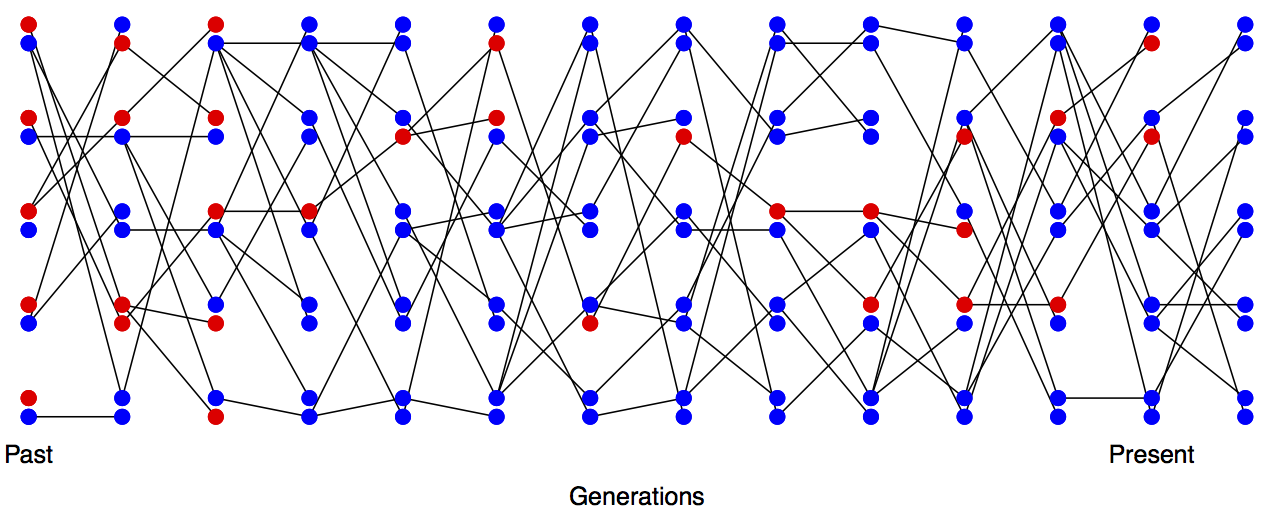
\includegraphics[width= \textwidth]{figures/Loss_of_he_col_two_alleles.png}
\end{center}
\caption{Loss of heterozygosity over time, in the absence of new
  mutations. A diploid population of 5 individuals over the
  generations, with lines showing transmission. In the first
  generation every individual is a heterozygote..} \label{fig:LossHet_two_alleles}
\end{figure} 

\begin{figure}
\begin{center}
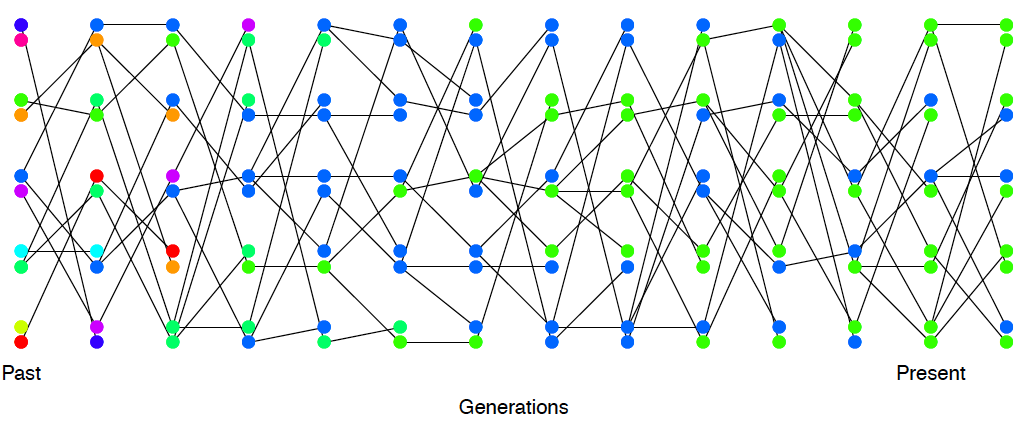
\includegraphics[width= \textwidth]{figures/Loss_of_het_2_many_alleles.png}
\end{center}
\caption{Loss of heterozygosity over time, in the absence of new
  mutations. A diploid population of 5 individuals. In the first generation I colour every allele a different
colour so we can track their descendants.} \label{fig:LossHet_many_alleles}
\end{figure} 



In the next generation ($t+1$) we are looking at the alleles in the
offspring of generation $t$. If we randomly sample two alleles in generation
$t+1$ which had different parental alleles in generation $t$ then it
is just like drawing two random alleles from generation $t$. So the
probability that these two alleles in generation $t+1$, that have
different parental alleles in generation $t$, are non-identical is
$H_t$. \\

Conversely, if our pair of alleles have the same parental allele in
the proceeding generation (i.e. the alleles are identical by descent
one generation back) then these two alleles must be identical (as we
are not allowing for any mutation). \\

In a diploid population of size $N$ individuals there are $2N$
alleles. The probability that our two alleles have the same parental
allele in the proceeding generation is $1/(2N)$, the probability that
they have different parental alleles is is $1-1/(2N)$. So by the above
argument the expected heterozygosity in generation $t+1$ is
\begin{equation}
H_{t+1} = \frac{1}{2N} \times 0 + \left(1-\frac{1}{2N} \right)H_t
\end{equation}
By this argument if the heterozygosity in generation $0$ is $H_0$ our
expected heterozygosity in generation $t$ is
\begin{equation}
H_t = \left(1-\frac{1}{2N} \right)^tH_0
\end{equation}
i.e. the expected heterozygosity with our population is decaying
geometrically with each passing generation. If we assume that $1/(2N)
\ll 1$ then we can approximate this geometric decay by an exponential
decay, such that
\begin{equation}
H_t =H_0 \exp \left(-\frac{t}{2N} \right)  
\end{equation}
i.e. heterozygosity decays exponentially at a rate $1/(2N)$.

\subsection{Levels of diversity maintained by a balance between
 mutation and drift} \label{DriftMutationBalance}

Looking backwards in time from one generation to the next, we are going
to say that two alleles which have the same parental allele (i.e. find
their common ancestor) in the
preceding generation have {\emph coalesced}, and refer to this event as a {\emph coalescent event}.

The probability that our pair of randomly sampled alleles have
coalesced in the preceding generation is $1/(2N)$, the probability
that our pair of alleles fail to coalesce is $1-1/(2N)$. 

The probability that a mutation changes the identity of the
transmitted allele is $\mu$ per generation. So the probability of no
mutation occurring is $(1-\mu)$. We'll assume that when a mutation
occurs it creates some new allelic type which is not present in the
population. This assumption (commonly called the infinitely-many-alleles model) makes the math slightly cleaner, and also
is not too bad an assumption biologically.

This model lets us calculate when our two alleles last shared a common
ancestor and whether these alleles are identical as a result of
failing to mutate since this shared ancestor.  For example we can work out the probability that our
two randomly sampled alleles coalesced $2$ generations in the past
(i.e. they fail to coalesce in generation $1$ and then coalescent in
generation $2$), and
that they are identical as
\begin{equation}
\left(1- \frac{1}{2N} \right) \frac{1}{2N} (1-\mu)^4
\end{equation}
note the power of $4$ is because our two alleles have to have failed
to mutate through $2$ meioses each.

More generally the probability that our alleles coalesce in generation
$t+1$ and are identical due to no mutation to either allele in the
subsequent generations is
\begin{equation}
P(\textrm{coal. in t+1 \& no mutations}) =  \frac{1}{2N} \left(1- \frac{1}{2N} \right)^t \left(1-\mu \right)^{2(t+1)}
\end{equation}
assuming that $\frac{1}{2N} \ll$ and $\mu \ll 1$ then we can
approximate this as
\begin{equation}
P(\textrm{coal. in t+1 \& no mutations}) \approx  \frac{1}{2N}
e^{-t/(2N)} e^{-2\mu (t+1)}
\end{equation}
to make this slightly easier on ourselves lets further assume that $t
\approx t+1$ and so rewrite this as
\begin{equation}
\approx \frac{1}{2N} e^{-t(2\mu+1/(2N))}
\end{equation}

\begin{figure}
\begin{center}
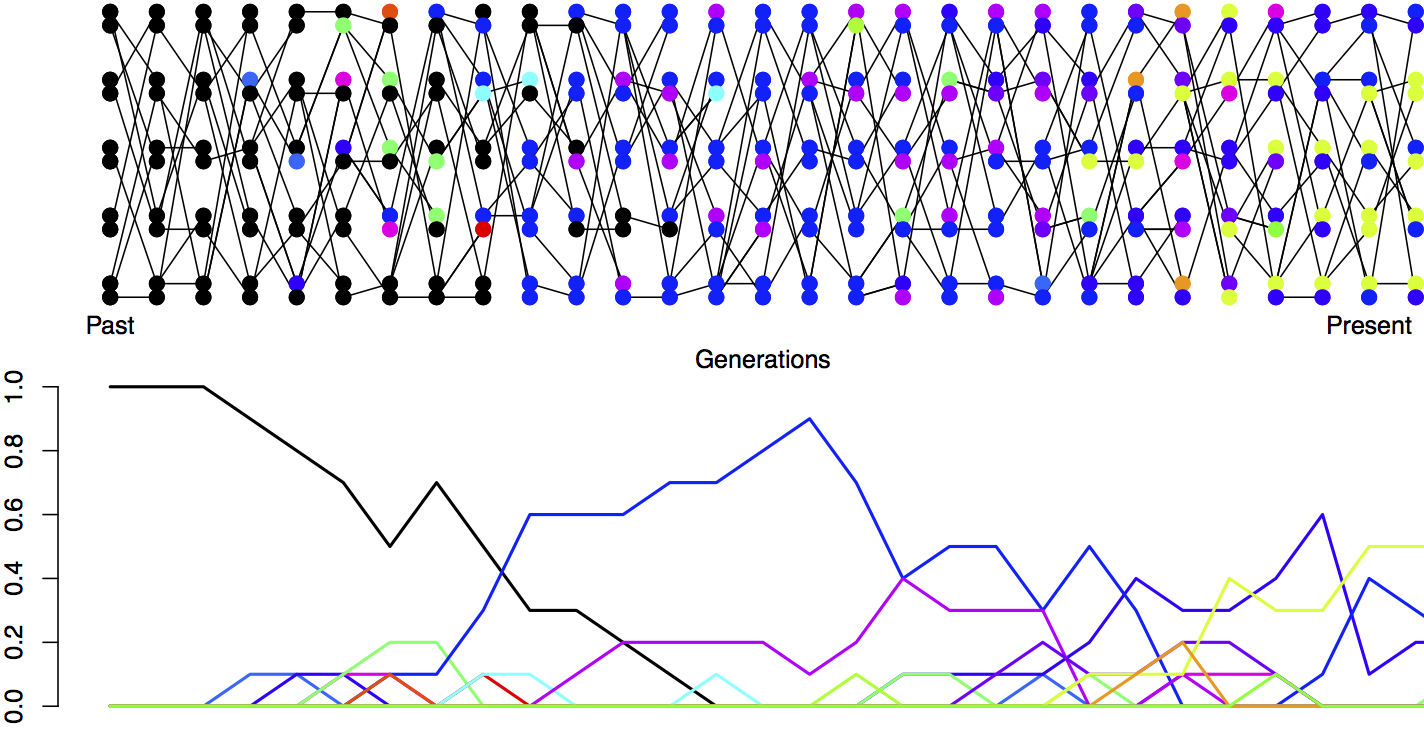
\includegraphics[width= 0.8 \textwidth]{figures/Mut_drift_balance}
\end{center}
\caption{Mutation-drift balance. A diploid population of 5
  individuals. In the first generation everyone has the same
  allele. Each generation the transmitted allele can mutate and we
  generate a new colour. In the bottom plot I trace the frequency of
  alleles in our population over time.} \label{fig:Mut_Sel_balance}
\end{figure} 

If we sample two alleles at random from the population we will not in
general know when they share a common ancestor. In which case we will
need to integrate out over when this coalescent event occurred. Doing
this we find the probability that our two alleles are identical due to
no mutation on either ancestral lineage since the pair shared a common
ancestor to be
\begin{equation}
\frac{1}{2N} \int_0^{\infty} e^{-t(2\mu+1/(2N))} dt =
\frac{1/(2N)}{1/(2N)+2\mu} = \frac{1}{1+4N\mu}
\end{equation}
The probability that our pair of alleles are non-identical is
simply one minus this, i.e.
\begin{equation}
\frac{4N\mu}{1+4N\mu} \label{eqn:hetero}
\end{equation}
This compound parameter $4N\mu$, the population-scaled mutation rate,
will come up a number of times so we'll give it its own name
\begin{equation}
\theta = 4N\mu
\end{equation}

So all else being equal, species with larger population sizes should
have proportionally higher levels of neutral polymorphism. 




\subsection{The effective population size.}
In practice populations rarely conform to our assumptions of being
constant in size with low variance in reproduction success. Real
populations experience dramatic fluctuations in size, and there is
often high variance in reproductive success. Thus rates of drift in
natural populations are often a lot higher than the census population
size would imply.\\

To cope with this population geneticists often invoke the concept of
an effective population size ($N_e$). In many situations (but not all), departures from model assumptions can be captured by substituting $N_e$ for $N$.

Specifically the effective population size ($N_e$) is the population
size that would result in the same rate of drift in an idealized constant
population size, obeying our modeling assumptions, as that observed in
our true population. \\

If population sizes vary rapidly in size, we can (if certain conditions are met)
replace our population size by the harmonic mean population size.
Consider a diploid population of variable size, whose size is $N_t$ $t$ generations into the
past. The probability our pairs of alleles have not coalesced by the generation $t^{th}$ is
given by
\begin{equation}
\prod_{i=1}^{t} \left(1-\frac{1}{2N_t} \right)
\end{equation}
note that this is simply collapses to our original expression
$\left(1-\frac{1}{2N } \right)^t $ if $N_i$ is constant. If $1/(N_i)$ is
small, then we can approximate $1-\frac{1}{2N_i}$ by
$\exp(-\frac{1}{2N_i})$. Such that if $N_i$ is never too small
\begin{equation}
\prod_{i=1}^{t} \left(1-\frac{1}{2N_i} \right)
\approx \prod_{i=1}^{t} \exp \left( -\frac{1}{2N_i} \right)   =
\exp \left(- \sum_{i=1}^{t} \frac{1}{2N_i} \right) .
\end{equation}
In our constant population size case
the probability of failing to coalesce is $\exp(-t/(2N))$. So the
variable population coalescent probabilities are still of the same form but
the exponent has changed. Comparing the exponent in the two cases we see
\begin{equation}
\frac{t}{2N} = \sum_{i=1}^{t} \frac{1}{2N_i}
\end{equation}
so that if we want a constant effective population size ($N_e$) that has the same
coalescent probability as our variable population we need to set
$N=N_e$ and rearrange this to see
\begin{equation}
N_e =\frac{1}{\frac{1}{t} \sum_{i=1}^{t} \frac{1}{N_i} }.
\end{equation}
this is the harmonic mean of the varying population size. Thus our
effective population size, the size of an idealized constant
population which matches the rate of genetic drift, is the harmonic
mean true population size over time. The harmonic mean is very
strongly affected by small values, such that if our population size is
one million $99\%$ of the time but drops to a $1000$ every hundred or
so generations, $N_e$ will be much closer to $1000$ than a million.\\

\begin{figure}
\begin{center}
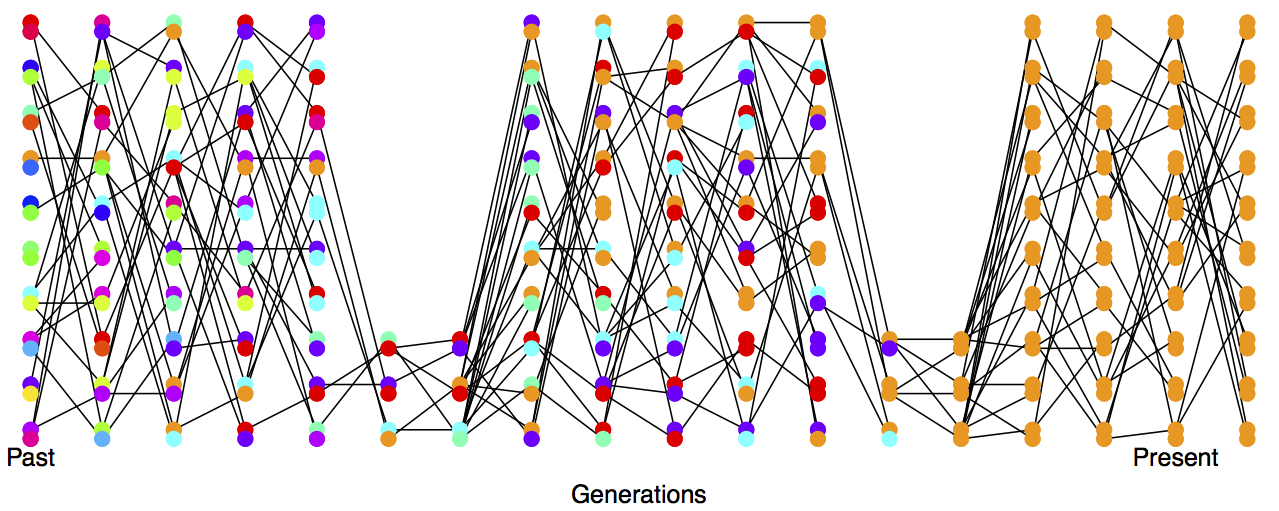
\includegraphics[width= \textwidth]{figures/Loss_of_he_col_alleles_varying_pop_dark.png}
\end{center}
\caption{Loss of heterozygosity over time in a bottlenecking population. A diploid population of 10 individuals, that bottlenecks
  down to three individuals repeatedly. In the first generation I colour every allele a different
colour so we can track their descendants, there are no new
  mutations.} \label{fig:LossHet_varying_pop}  
\end{figure} 

%would result in the same rate of drift
%Luckily, in many (not all) situations, departures from model assumptions can be captured by substituting Ne for N, i.e., by plugging in a fictitious N that leads to the same level of genetic drift as observed.

Variance in reproductive success will also affect our effective
population size. Even if our population has a large constant size of $N$
individuals, if only small proportion of them get to reproduce then
the rate of drift will reflect this much small number of reproducing
individuals. If only $N_M$ males get to contribute to the next
generation and $N_F$ females get to contribute to the next
generation. When our two alleles pick an ancestor, $25\%$ of the time
our alleles were both in a female ancestor in which case they coalesce
with probability $1/(2N_F)$, and $25\%$ of the time they are both in a
male ancestor in which case they coalesce with probability
$1/(2N_M)$. The remaining $50\%$ of the time our ancestral lineages
are in two individuals are different sexes in a generation so cannot
coalescence.  Therefore, our probability of coalescence in the preceding
generation is
\begin{equation}
\frac{1}{4}\frac{1}{2N_M}+\frac{1}{4}\frac{1}{2N_F} =
\frac{1}{8}\frac{N_F+N_M}{N_FN_M} 
\end{equation}
i.e. the rate of coalescence is the harmonic mean of the two
sexes population sizes, 
equating this to $\frac{1}{2N_e}$ we find
\begin{equation}
N_e = \frac{4N_FN_M}{N_F+N_M}
\end{equation}
Thus if reproductive success is very skewed in one sex (e.g. $N_M \ll
N/2$) our effective population size will be much reduced as a result.\\


\begin{figure}
\begin{center}
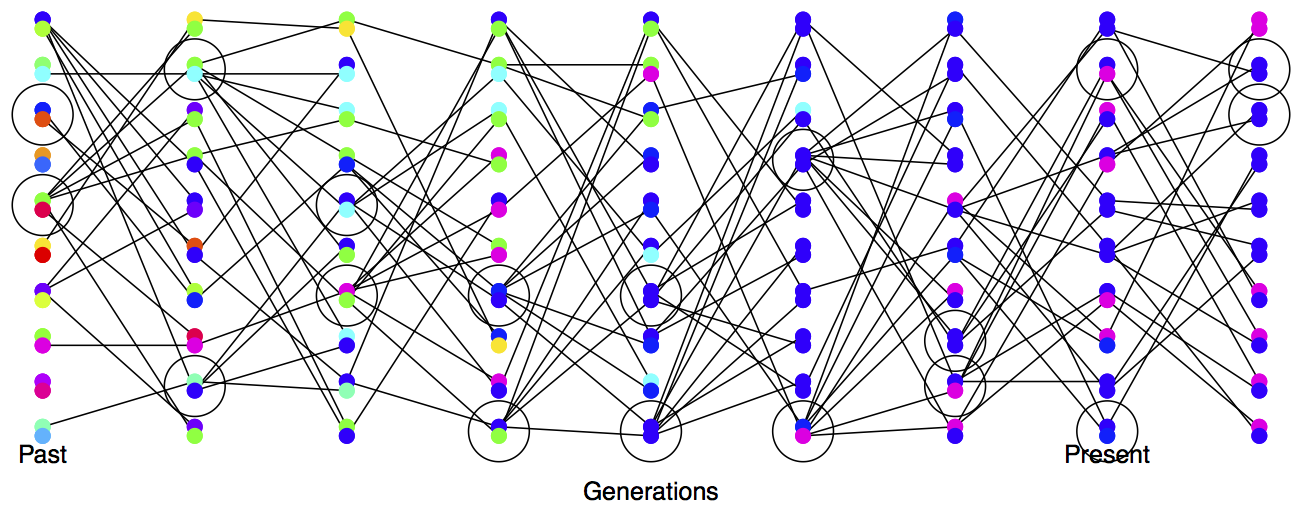
\includegraphics[width= \textwidth]{figures/Loss_of_he_col_alleles_varying_RS.png}

\end{center}
\caption{High variance on reproductive success increases the rate of genetic drift. A diploid population of 10 individuals, where the circled
  individuals have much higher reproductive success. In the first generation I colour every allele a different
colour so we can track their descendants, there are no new
  mutations.} \label{fig:LossHet_varying_RS}
\end{figure} 

\subsection{Neutral diversity and population structure}
%%this section was moved from the coalescent chapter
Upto now we have assumed that our alleles that we have modelled in the
coalescent setting are drawn from a randomly mating population such
that any pair of lineages is equally likely to coalesce with each
other. However, when there is population structure this assumption is
violated. \\

We have previously written the measure of population structure
$\fst$ as
\begin{equation}
\fst = \frac{H_T-H_S}{H_T}
\end{equation}
where $H_S$ is the probability that two alleles sampled at random from a
subpopulation differ, and $H_T$ is the probability that two alleles
sampled at random from the total population differ. 

\paragraph{A simple population split model}
Imagine a population of constant size of $N_e$ diploid individuals that
$\tau$ generations in the past split into two daughter populations (sub-populations)
each of size $N_e$ individuals, who do not subsequently exchange
migrants. In the current day we sample an equal number of alleles
from both subpopulations.

Consider a pair of alleles sampled within one of our
sub-populations, they have experienced a population of size $N_e$
and so the probability that they differ is $H_S = \theta/(1+\theta)$
(where $\theta=4N_e\mu$).
The heterozygosity in our total population is a little more tricky to
calculate. Assuming that we equally sample both sub-populations, when we draw two alleles from our total
sample, $50\%$ of the time they are drawn from the same
subpopulation and $50\%$ of the time they are drawn from different
subpopulations. Therefore, our total heterozygosity is given by
\begin{equation}
H_T = \half H_S + \half H_B
\end{equation}
where $H_B$ is the probability that a pair of alleles drawn from our
two different sub-populations differ from each other. Our pair of
alleles can not find a common ancestor with each other for at least $\tau$
generations into he past as they are in distinct populations (not
connected by migration). The probability that one or other of them
mutates in this time is $1-(1-\mu)^{2T}$. With probability
$(1-\mu)^{2T} $ neither of our alleles mutate in the $T$ generations
back in time before they find themselves back in the combined ancestral 
population. Conditional on failing to mutating before the combined ancestral
population, the probability that they do manage to mutate before
coalescing in that population of size $N_e$ is
$\theta/(\theta+1)$. Putting these components together
\begin{equation}
H_B = \left( 1-(1-\mu)^{2T} \right) + (1-\mu)^{2T}
  \frac{\theta}{\theta+1} 
\end{equation}
We can plug this into our expression for $H_T$, and then that in turn
into $\fst$.

\begin{figure}
\begin{center}
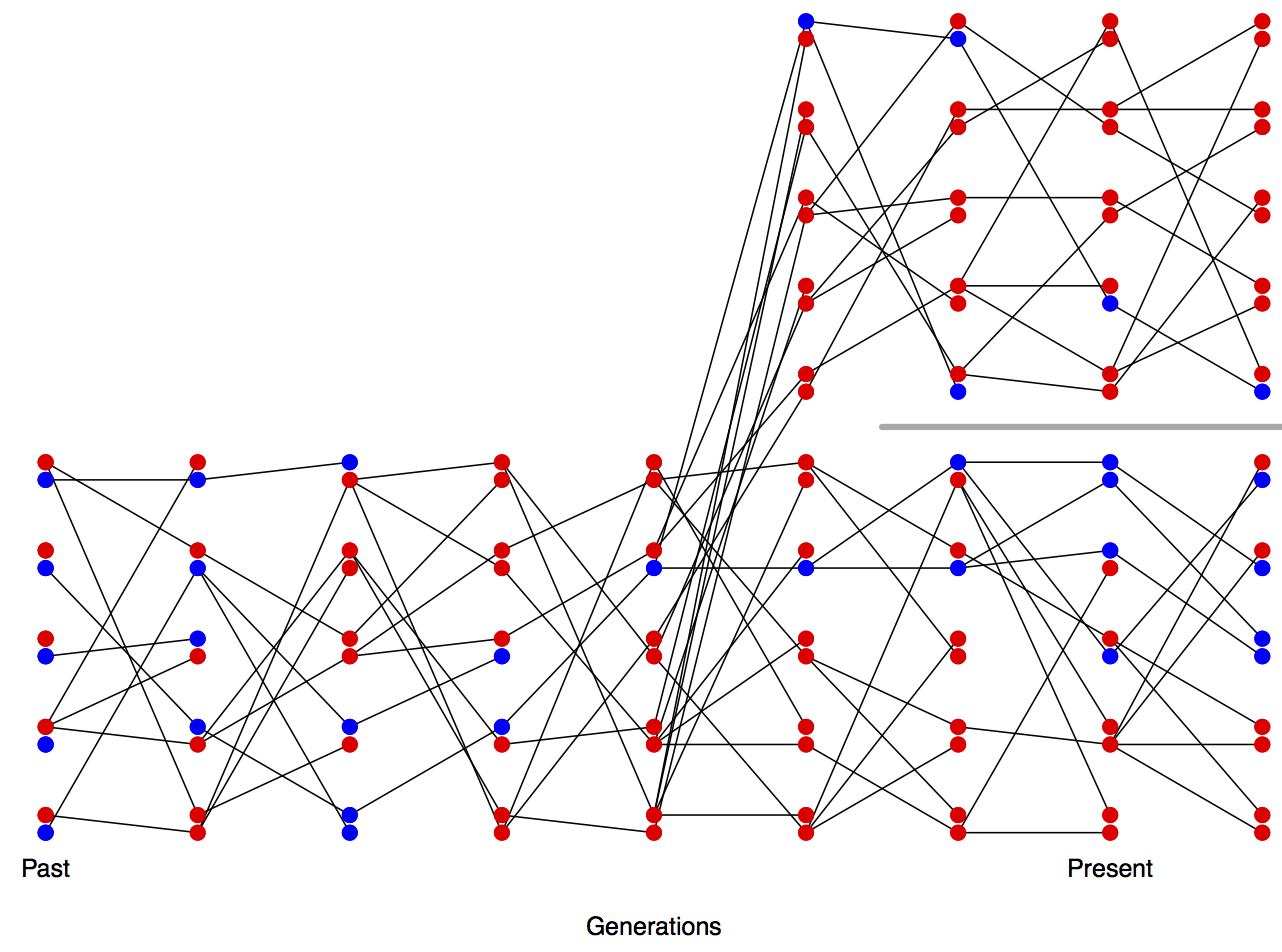
\includegraphics[width= 0.8 \textwidth]{figures/drift_split.png}
\end{center}
\caption{Change in allele frequencies following a population split.} \label{fig:drift_split}  
\end{figure} 

To understand this better we can make a simple
approximation based on our mutation rate being very low, such that
$N_e \mu \ll 1$ ao $H_S \approx
4N_e\mu$, and that $\mu \ll 1$ and $\mu T \ll 1$. Assuming this, then  
\begin{equation}
H_B \approx 2 \mu T + 4N_e\mu. 
\end{equation}
So that 
\begin{equation}
\fst \approx \frac{ \mu T}{\mu T +  4N_e\mu }  %= \frac{ T}{ T +  4N_e }
\end{equation}
note that $\mu$ cancels out of this. In this simple toy model $\fst$
is increasing because the amount of between population diversity 
increases with the divergence time of the two populations (initially
linearly with $T$). It does so at a rate
give by $T/(4N_e)$ so that differentiation will be higher
between populations separated by long divergence times or with small
effective population sizes.

\paragraph{A simple model of migration between an island and the mainland.}
We can also use the coalescent to think about patterns of
differentiation under a simple model of migration drift
equilibrium. Lets consider a small island population that is relatively isolated
from a large mainland population, and that both of these populations
are constant in size. We'll assume that the expected heterozygosity
for a pair of alleles sampled on the mainland is $H_M$.

Our island has a population size
$N_{I}$ that is very small compared to our mainland population.
Each generation some low fraction $m$ of our individuals on the
island have migrant parents from the mainland the generation
before. Our island may also send migrants back to the mainland, but
these are a drop in the ocean compared to the large population size on
the mainland and their effect can be ignored. 


If we sample an allele on the island back and trace its ancestral
lineage backward in time, each generation our ancestral allele have a low
probability $m$ of being descended from the mainland in the proceeding
generation (if we go far enough the allele eventually has to be
descended from an allele on the mainland). The probability that a pair of alleles sampled on the
island are descended from a shared recent common ancestral allele on the island, is the
probability that our pair of alleles coalesce before either lineage
migrates. For example, the probability that our pair of alleles
coalesce $t+1$ generations back is 
\begin{equation}
\frac{1}{2N_I}(1-m)^{2(t+1)} \left(1-\frac{1}{2N_I} \right)^{t} \approx
\frac{1}{2N_I} \exp\left( -t\left (\frac{1}{2N_I} + 2m\right) \right),
\end{equation}
with the approximation following from assuming that $m \ll 1$ \& $1/(2N_I)
\ll 1$ (note that this is very similar to our derivation of
heterozygosity above). The probability that our alleles coalescence before either one
of them migrates off the island, irrespective of the time, is
\begin{equation}
\int_0^{\infty} \frac{1}{2N_I} \exp\left( -t\left (\frac{1}{2N_I} +
    2m\right) \right) dt = \frac{1/(2N_I) }{1/(2N_I) +
    2m}.
\end{equation}

Lets assume that the mutation rate is very low such as it is very
unlikely that the pair of alleles mutate before they coalesce on the
island. Therefore, the only way that the alleles can be different from
each other is if one or other of them migrates to the mainland, which
happens with probability  
\begin{equation}
1 - \frac{1/(2N_I) }{1/(2N_I) + 2m}
\end{equation}
Conditional on one or other of our alleles migrating to the mainland,
both of our alleles represent independent draws from the mainland and
so differ from each other with probability $H_M$. Therefore, the level of
heterozygosity on the island is given by
\begin{equation}
H_I = (1 - \frac{1/(2N_I) }{1/(2N_I) + 2m})H_M
\end{equation}
So the reduction of heterozygosity on the island compared to the
mainland is
\begin{equation}
F_{IM} = 1- \frac{H_I}{H_M} = \frac{ 1/(2N_I) }{1/(2N_I) + 2m} = \frac{ 1 }{1 + 4N_Im}.
\end{equation}
The level of inbreeding on the island compared to the mainland will
be high in the migration rate is low and the effective population size
of the island is low, as allele frequencies on the island are drifting
and diversity is not being replenished on the island by migration. The
key parameter here is the number individuals on the island replaced by
immigrants from the mainland each generation ($N_I m$).

We have framed this as being about the reduction in genetic diversity on the
island compared to the mainland. However, if we consider collecting a
individuals on the island and mainland in proportion to population
sizes the total level of heterozygosity would be $H_T=H_M$, as samples
from our mainland would greatly outnumber those from our
island. Therefore, considering our island our sub-population we have
derived another simple model of $F_{ST}$ .


\newpage

